% !TEX root = /Users/saxer/Documents/uppsalaDV/pkd/project/Cashier-System/Report.tex
% !TEX encoding = UTF-8 Unicode
\documentclass[11pt]{article}
\usepackage[a4paper,top=3cm,bottom=2cm,left=3cm,right=3cm,marginparwidth=1.75cm]{geometry}
\usepackage[T1]{fontenc}
\usepackage[utf8]{inputenc}
\usepackage[english]{babel}
\usepackage{graphicx}
\usepackage{listings}
\usepackage{color}

\lstset{
  frame=none,
  xleftmargin=2pt,
  stepnumber=1,
  numbers=left,
  numbersep=5pt,
  numberstyle=\ttfamily\tiny\color[gray]{0.3},
  belowcaptionskip=\bigskipamount,
  captionpos=b,
  escapeinside={*'}{'*},
  language=haskell,
  tabsize=2,
  emphstyle={\bf},
  commentstyle=\it,
  stringstyle=\mdseries\rmfamily,
  showspaces=false,
  keywordstyle=\bfseries\rmfamily,
  columns=flexible,
  basicstyle=\small\sffamily,
  showstringspaces=false,
  morecomment=[l]\%,
}

\begin{document}
\title{Project - Business register and database}
\author{Group 23: Jesper Saxer, Sebastian Lhådö , Grim Moström}
\date{\today}
\maketitle{}
\section{Introduction}
Conducting business on a professional level can be overwhelming without the proper tools and systems. It is essential that business actions and cash flows are tracked. Without  a functional system it can be complicated to trace how eventual mistakes or disadvantageous business actions are affecting the business and even worse, to track inventories and cash flows during the declaration of taxes. A proper business tool such as a Business register can be helpful to administrate multiple users in the business in order to keep track of actions and cash flows. This project aims to create a complete system that keeps track of stock, purchases, identification of users and most importantly the in and outgoing cash flows. In addition it also provides a customer based cart system in order to help the customer, improving the total user experience, assisting the customer in the decision and payment process.
\pagebreak
\tableofcontents
\pagebreak
\section{Illustration of the Business system}
In order to deliver a complete understanding of the business system, we have chosen to map our system in graphical context. This way we can guide the reader through the build of the system and it’s hidden functions.\\\\
The following graphical summary is a brief summary of the main functions of the business computer system.
\section{Flow chart}
\begin{figure}[h]
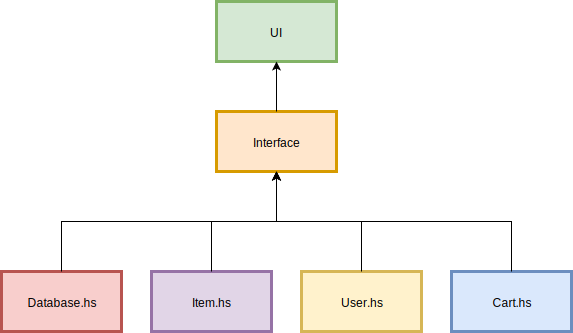
\includegraphics[width=\linewidth]{FlowChart.png}
\caption{Flow chart over the shop}
\label{fig:flow chart}
\end{figure}
\section{Branch declarations}
\subsection{Database}
The database administrates and stores the main functions in its context. Through this system we can store the inventory, create users, and receive purchases or changes in stock.
The database is functioning as an information bank in which information can be edited such that it fits the needs of the administrator, thus correlating to the reality of the business process conducted externally in practice. Without the database, it is impossible to store the information that has been put into the system. This implies that it is an essential piece of the complete business system.\\\\
Please read further in Branch \& Data structure specification X:X for further information
\pagebreak
\subsection{User}
When registering business-transactions it is important for the system to determine whether the user is an administrator, employee or a customer in order to offer the right services and properties.
The system is designed such that it offers an administrator the full access to change all variables in the system, including the users available to administer the system.
An employee has the same properties as an administrator, except for user and item administration. Thus, an employee is not able to remove users from the program, as well as items. However, an employee is able to manage stock and properties of customers, in order to remove inappropriate usage or incorrect repository values.\\\\
Please read further in Branch \& Data structure specification X:X for further information
\subsection{Item}
One of the most essential parts of the business system is the Item specification. The items builds unit specification on purchasable goods in the system. Further you upload one of these items to the database in order to sync it to the active transaction flows and stock rates. An item holds all the needed information to specify the products values, such as the stock, EAN code, price, and name. \\\\
Please read further in Branch \& Data structure specification X:X for further information
\subsection{Cart}
The cart is a temporary list of chosen products by the User.  This cart holds products in order to sum up the list of chosen products and giving the user a sum of total cost.
From here it is easy to navigate in order to add more products or remove them. This way the usability of the system increases since the customer can iterate the shopping list while being able to keep on shopping. \\\\
Please read further in Branch \& Data structure specification X:X for further information
\subsection{Interface}
\subsubsection{Functional Interface}
The interface is divided in two levels of functionality. The function interface, and the graphical interface.
Interface functions is our gathering channel from our systems flow chart. This is the channel in which the User interacts with the complete business system. By hiding all help functions in the back end systems you can easily communicate in a front-end manor to the user, simplifying the systems usability, improving the user experience. This way we enable the customer to handle the system without any further practical guidance than what is offered by the business system itself. \\\\
Please read further in Branch \& Data structure specificationX:X for further information
\subsubsection{Graphical Interface}
The graphical interface is a visualization of the interface functions to get the complete front-end product. With a graphical interface the User is furtherly being guided in the useage of the system. This is the final level of the product, surfacing to the interaction with the User.\\\\
Please read further in Branch \& Data structure specification specification X:X for further information
\section{Branch \& Data structure specification}
\subsection{Database}
Database.hs is the way we choose to represent a Database in our Cashier-System. Our Database.hs has its own datatypes which is defined the following preset:
\begin{lstlisting}
type Id = Int -- Ean for item, userId for users
\end{lstlisting}

Explanation: The identity of a user is defined by a User code, based on integers. These numbers are unique for each User and makes  it easy to identify two different users with similar names.
The identity of Items are identified by a corresponding, or matching EAN code, scanned on the products back. This serial code defines the sort of product and is unique for the specific type of product specified.
\begin{lstlisting}
type Database a = [(a,Id)]
\end{lstlisting}

The data type Database is polymorphic. This implicates that it is non type specific.  This way, Database can hold both user identities and items. This is fitting to the needs of information storage to be held in the business system. In summarization the Database takes one polymorphic argument and returns a tuple containing this argument together with an ID.\\\\
The following functions are reachable if Database.hs is imported
\begin{lstlisting}
empty :: Database a
deleteWithID :: Id -> Database a -> Database a
insert :: a -> Id -> Database a -> Database a
grabWithID :: Id -> Database a -> a
\end{lstlisting}

Notation: In the structure of the function specifications for the functions above. You can see a collection of types with an arrow pointing right. The value presented after the last arrow indicates what the complete function returns. The other arrows is simply separating arguments that the function takes while being called!\\\\
The same fundamental constructional frame of functions is maintained through the whole project.
\pagebreak
\subsection{User}
User.hs is the representation of User identities in the Cashier-System. Our User.hs has its own data structure which is defined in the following way.
\begin{lstlisting}
type Name = String
type Id = Int
type Wallet = Int
type Spent = Int
type IsAdmin = Bool

data User = User Name Id Wallet Spent IsAdmin deriving (Show, Eq)
\end{lstlisting}

This implicates that every User takes the following Arguments…
Name is represented by a String of characters bound between two “ ” symbols.
Example: “Name”\\
Id, is represented by a series of numbers, identifying the user by unique numerical identification by integers.\\
Example: Id “Sebastian” = 1234\\
Wallet: The Wallet is a data type representing the amount of money a user have stored in the system. This virtual money represented by integers is later at disposal on the products put into the system.\\
Spent represents the amount of money a user have spent in our shop. The purpose of this datatype is to track cashflows in the system and follow up on the systems revenues.\\
IsAdmin keeps tracks the user itself have admin properties or not. This is very important in order to keep the business systems integrity level. By having administrator properties, the system disables customers access to sensitive data and essential product maintenance functions.\\\\
The following functions are reachable if User.hs is imported.
\begin{lstlisting}
newUser       :: Name   -> Id   -> Wallet -> Spent -> IsAdmin -> User
setName       :: Name   -> User -> User
getName       :: User   -> Name
setId         :: Id     -> User -> User
getId         :: User   -> Id
fillWallet    :: Wallet -> User -> User
removeWallet  :: Wallet -> User -> User
removeSpent   :: User   -> User
makeAdmin     :: User   -> User
removeAdmin   :: User   -> User
addSpent      :: Spent  -> User -> User
getWallet     :: User   -> Wallet
clearWallet   :: User   -> User
\end{lstlisting}

\subsection{item}
\subsection{Cart}
\subsection{Interface}
\subsubsection{Functional Interface}
\subsubsection{Graphical Interface}
\section{User Guide}
\section{User cases}
\section{Algorithms}
\subsection{Recursive algorithms}
\subsection{Pattern matching}
\section{Tests \& Debugging}
\section{Shortcomings of the program}










\end{document}
